\documentclass[12pt]{article}

\usepackage[a4paper,margin=2.5cm]{geometry}
\usepackage{amsmath, amssymb, amsthm}
\usepackage{bm}
\usepackage{hyperref}
\usepackage{graphicx}
\usepackage{caption}
\usepackage{listings}
\usepackage{xcolor}
\usepackage{float}
\usepackage{placeins}
\graphicspath{{figures/}}

\lstdefinestyle{code}{
  basicstyle=\ttfamily\small,
  numbers=left,
  numberstyle=\tiny,
  numbersep=8pt,
  keywordstyle=\color{blue},
  commentstyle=\color{teal!70!black},
  stringstyle=\color{orange!70!black},
  showstringspaces=false,
  breaklines=true,
  frame=single,
  framerule=0.3pt,
  rulecolor=\color{black!15}
}
\lstset{style=code}

\title{Isolation Forest Tutorial}
\author{}
\date{\today}

\begin{document}
\maketitle

\section{Introduction}
Isolation Forest detects anomalies by randomly partitioning data points until they become isolated. Unlike density-based approaches, it relies on the observation that anomalies are easier to isolate due to their sparsity and feature-wise extremity. The algorithm builds an ensemble of random trees, yielding scores that quantify how anomalous each observation is.

\section{Theory and Formulas}
\subsection{Random Partitioning}
Each isolation tree is grown by recursively selecting a random feature and a random split value within its range. For a sample \(\mathbf{x}\), the path length \(h(\mathbf{x})\) equals the number of edges traversed from the root to the external node containing \(\mathbf{x}\). Anomalies typically have shorter path lengths, while normal points require more splits to isolate.

\subsection{Path Length and Anomaly Score}
For a subsample size \(\psi\), the average path length of unsuccessful searches in a Binary Search Tree is
\begin{equation}
\mathbb{E}[h(\psi)] = 2 H_{\psi-1} - \frac{2(\psi-1)}{\psi}, \qquad H_n = \sum_{k=1}^n \frac{1}{k}.
\end{equation}
The anomaly score for \(\mathbf{x}\) is
\begin{equation}
s(\mathbf{x}, \psi) = 2^{-\frac{\overline{h(\mathbf{x})}}{\mathbb{E}[h(\psi)]}},
\end{equation}
where \(\overline{h(\mathbf{x})}\) is the average path length across all trees. Scores near 1 indicate strong anomalies; scores below 0.5 are likely normal.

\subsection{Hyperparameters and Complexity}
Key parameters include the number of estimators, subsample size, and contamination ratio that calibrates the decision threshold. Isolation Forest runs in \(O(t \psi \log \psi)\) time for \(t\) trees with subsample size \(\psi\), offering linear scalability in the number of samples and features. Feature scaling and handling categorical variables are crucial for meaningful splits.

\section{Applications and Tips}
\begin{itemize}
  \item \textbf{Fraud detection}: surface unusual transactions in finance or e-commerce.
  \item \textbf{Network security}: detect rare traffic signatures in high-dimensional logs.
  \item \textbf{Manufacturing}: flag sensor readings that deviate sharply from normal operating patterns.
  \item \textbf{Best practices}: standardize features, tune subsample size and contamination, inspect score distributions, and combine with domain knowledge to validate alerts.
\end{itemize}

\section{Python Practice}
The script \texttt{gen\_isolation\_forest\_figures.py} creates synthetic data with injected anomalies, fits scikit-learn's IsolationForest, and visualizes anomaly scores over the feature space along with a histogram highlighting detected outliers.
\begin{lstlisting}[language=Python,caption={Excerpt from gen_isolation_forest_figures.py}]
from sklearn.ensemble import IsolationForest

model = IsolationForest(
    n_estimators=200,
    max_samples=256,
    contamination=0.08,
    random_state=42,
)
model.fit(points)
score = model.decision_function(points)
labels = model.predict(points)
\end{lstlisting}

\section{Result}
\begin{figure}[H]
  \centering
  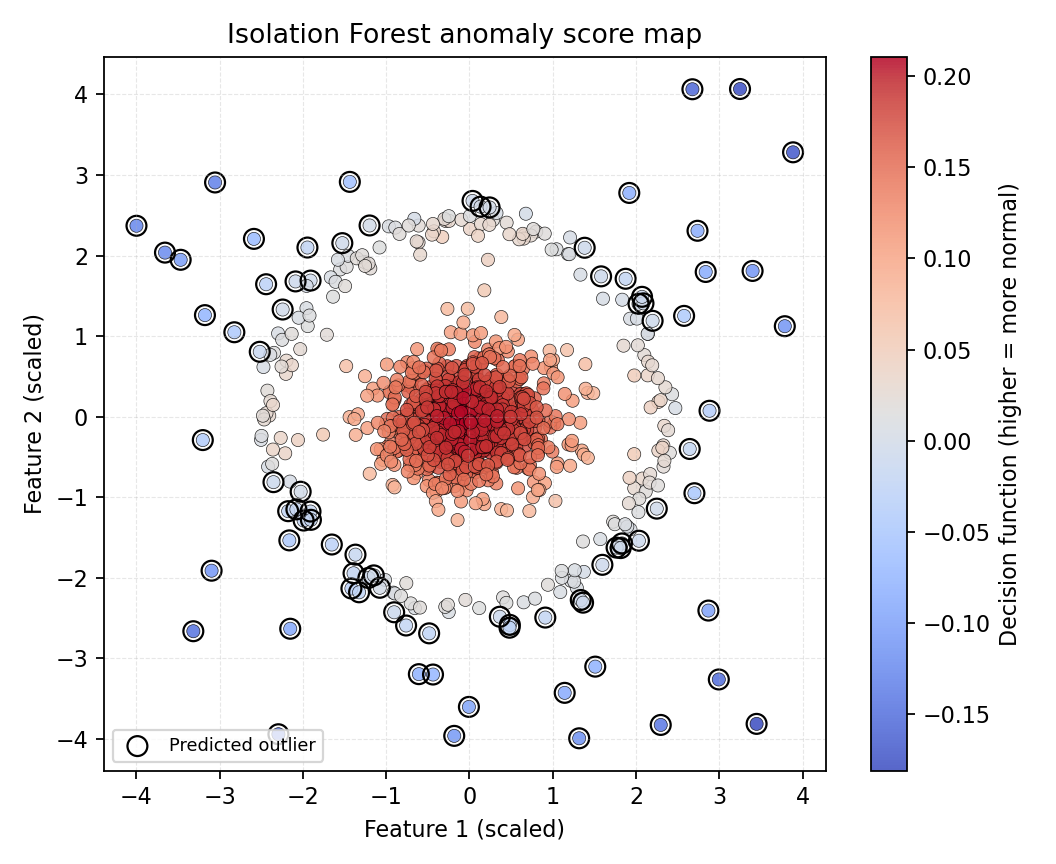
\includegraphics[width=0.82\linewidth]{isolation_forest_decision.png}
  \caption{Isolation Forest anomaly scores on synthetic data; darker regions indicate higher anomaly likelihood}
  \label{fig:isolation_forest_decision}
\end{figure}

\begin{figure}[H]
  \centering
  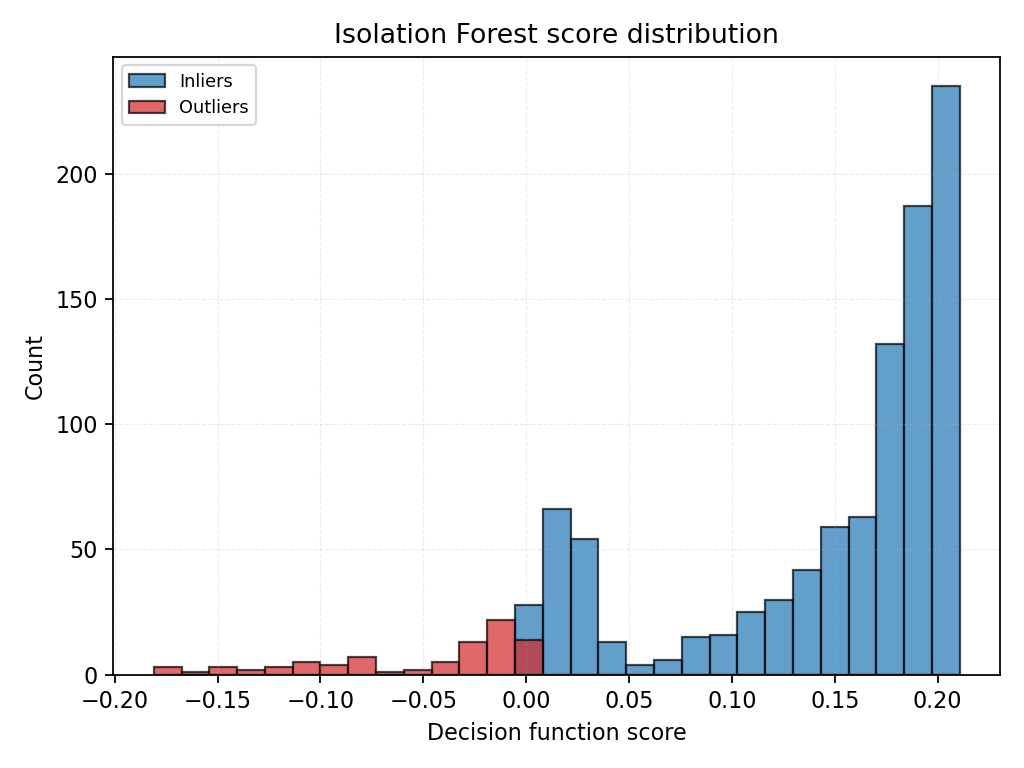
\includegraphics[width=0.78\linewidth]{isolation_forest_score_hist.png}
  \caption{Histogram of anomaly scores separating predicted inliers and outliers}
  \label{fig:isolation_forest_score_hist}
\end{figure}

\FloatBarrier
\section{Summary}
Isolation Forest isolates anomalies via random splits, producing interpretable scores with few assumptions about data distribution. Proper feature scaling and parameter tuning yield robust detectors for high-dimensional datasets. The synthetic example demonstrates how score visualizations validate threshold choices and highlight anomalous clusters.

\end{document}